\chapter{New Concepts}
\label{chp_new_concepts}
The XGEE visualization verification algorithms are essential for interpreting and optimizing diagram structures within the editor.
While the original implementations demonstrated functionality in basic test cases, their limitations prevented comprehensive detection across various diagram types and complexities. This chapter introduces enhanced methods to address these limitations and significantly increase detection accuracy, versatility and stability.
\section{Edge Detection}
\label{chp_edge_detection}
Edges represent connections between vertices, inputs and outputs. Detecting edges accurately requires an approach that can identify individual line segments and how they connect to form complex chains. This section introduces a robust edge detection pipeline leveraging multiple computer vision techniques to reliably identify edges across a wide variety of block diagrams within XGEE.

\subsection{Methology}
\begin{wrapfigure}{R}{0.4\textwidth}
    \centering
    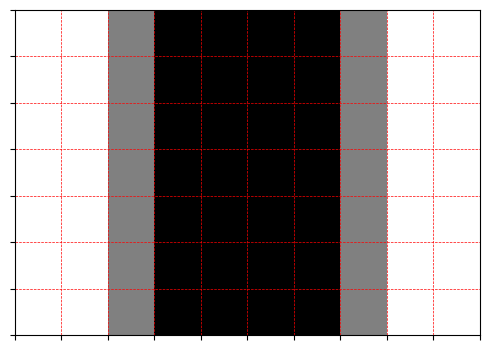
\includegraphics[width=\linewidth]{Pictures/kernel_ver.png}
    \caption{kernel for vertical edges}
    \label{fig_kernel_ver}
\end{wrapfigure}
Since there are only vertical and horizontal edges within XGEE, two kernels will be used to find all pixels containing either part of a vertical or horizontal edge. The \textit{filter2D()} function places the kernel anchor (usually the top left value of the kernel) on top of a pixel, with the rest of the kernel overlapping the corresponding local pixels.\\
The kernel values are then multiplied by the corresponding pixel values underneath and added together. The result is saved and placed on the location of the anchor. The kernel on the right \ref{fig_kernel_ver} is rotated by 90\textdegree  to generate the horizontal kernel. The same process can be written as equation \ref{eq_filter2D}, where \(H\) is the resulting matrix, \(I\) is the original image and \(K\) is the used kernel. This process is repeated for every pixel and, depending on the structure of the kernel, it can also be used to blur or sharpen an image \cite{web_filter2D}.\\
Each value in the processed image is normalized to an 8-bit integer between 0 and 255. This allows the data to be visualized as a gray scale image \ref{fig_filter2d} and processed using OpenCV's \textit{threshholding()} function \ref{fig_threshhold}. As illustrated in figure \ref{fig_comparison_filter}, ports and letters are sometimes misidentified as edges. Additionally, intersections of edges and points where horizontal and vertical edges meet are not immediately detected. These challenging areas will be processed individually in a later step in the edge detection pipeline. Apart from these specific cases, the method effectively extracts all pixels corresponding to vertical and horizontal edges, provided their widths match those of the used kernels.
\begin{equation}
\label{eq_filter2D}
    H(x, y) = \sum_{i=0}^{M_i-1} \sum_{j=0}^{M_j-1} I(x + i - a_i,y + j - a_j)K(i, j)
\end{equation}\\

\newpage

\begin{figure}[htb]
    \centering
    \includegraphics[width=1\linewidth]{Pictures/filter2D.png}
    \caption{Filter2D function results}
    \label{fig_filter2d}

    \centering
    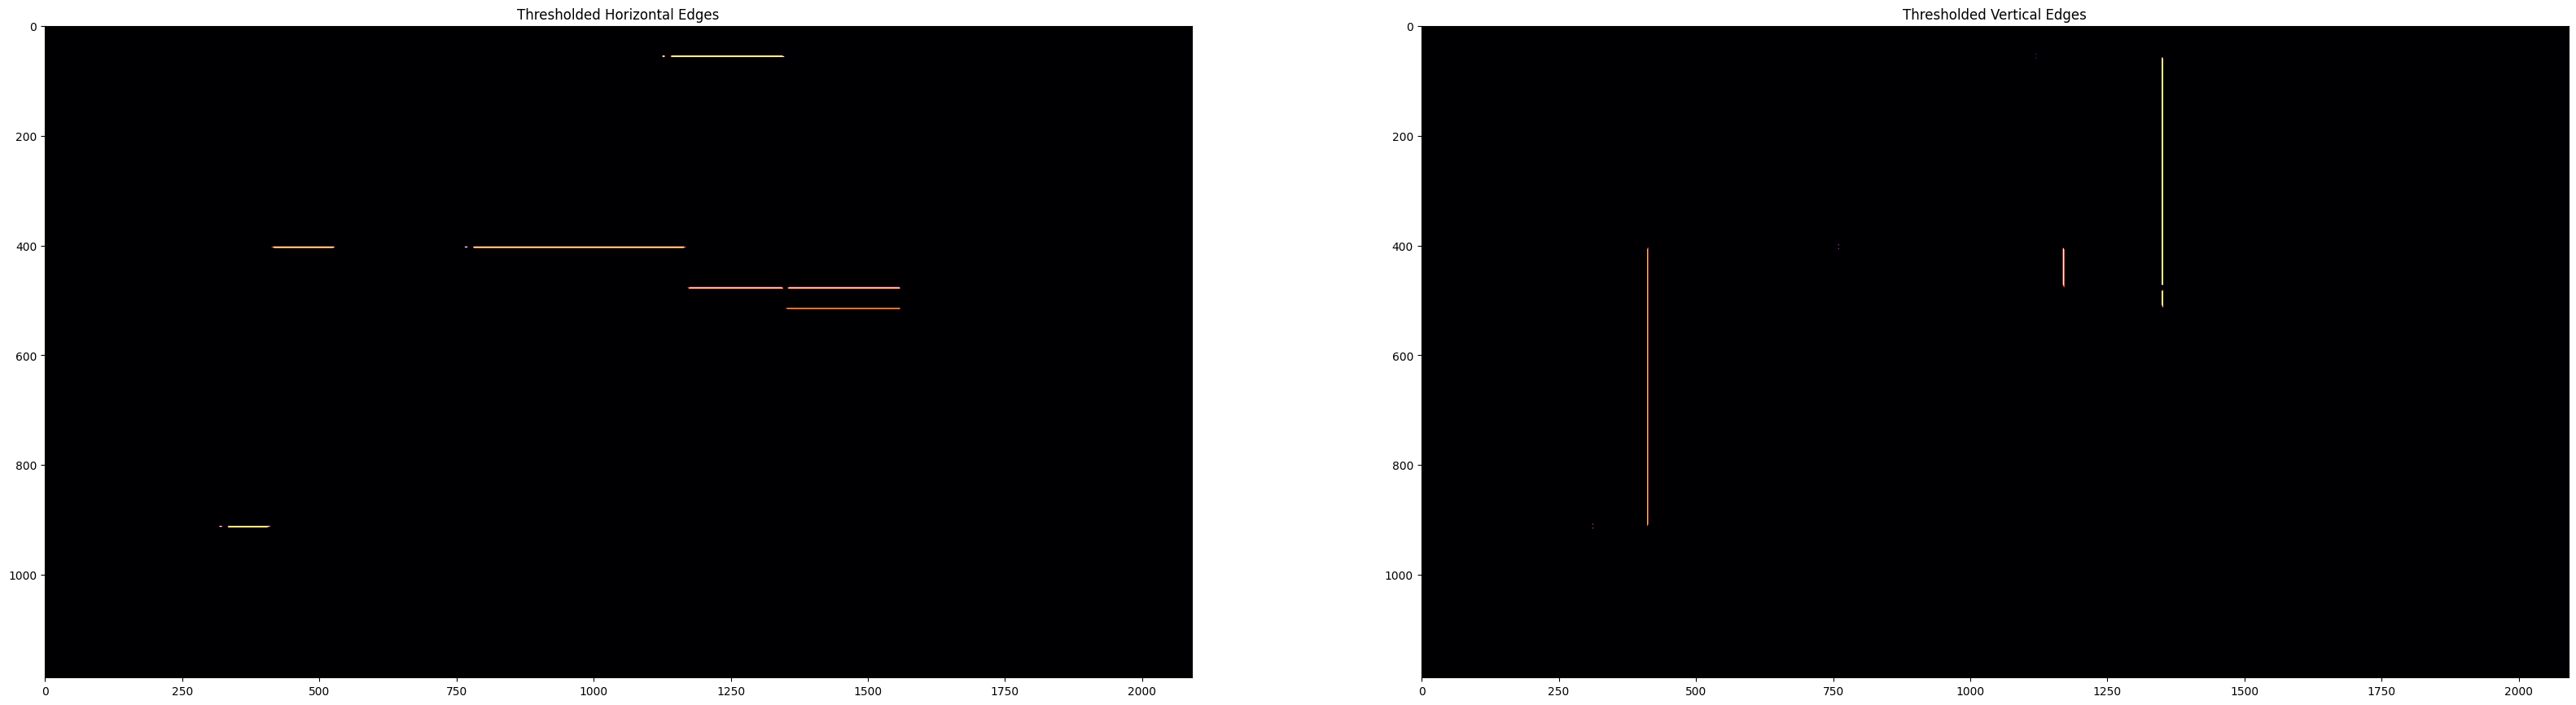
\includegraphics[width=1\linewidth]{Pictures/threshhold.png}
    \caption{Threshholded filter2D function results}
    \label{fig_threshhold}
\end{figure}
For easier processing and data storage, the threshholded pixels \ref{fig_threshhold} are converted to line segments consisting of start- and endpoints. This is achieved through two of OpenCV's built-in functions:\\
\textit{findContours()}, which retrieves contours from a binary image using an algorithm introduced in this paper: \cite{art_findContours()_algorithm}.\\
\textit{approxPolyDP()}, which approximates a curve or a polygon with another curve or polygon with less vertices using an algorithm introduced in this paper: \cite{art_approx_Poly_DP()_algorithm}.
\begin{figure}[h]
  \centering
  \begin{minipage}[b]{0.45\textwidth}
    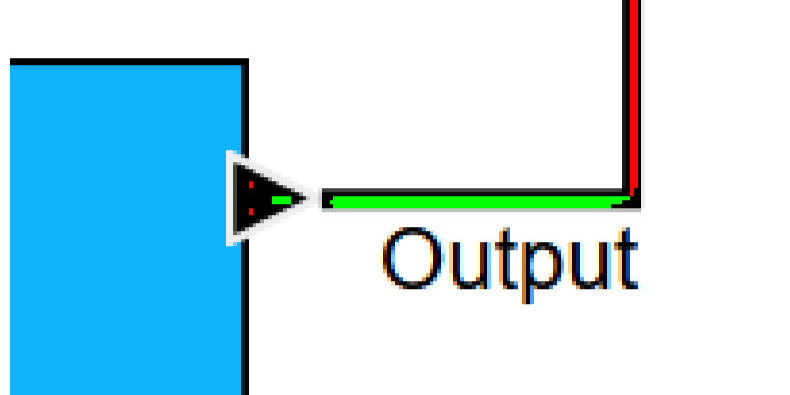
\includegraphics[width=\textwidth]{Pictures/thresh_zoom.png}
  \end{minipage}
  \hfill
  \begin{minipage}[b]{0.45\textwidth}
    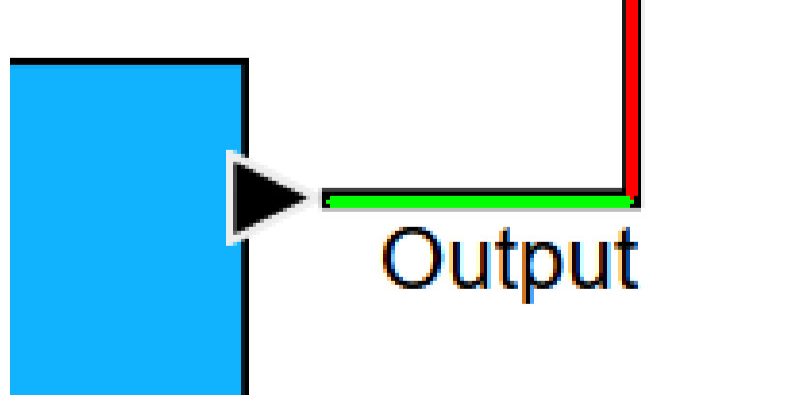
\includegraphics[width=\textwidth]{Pictures/line_segments_zoom.png}
  \end{minipage}
  \caption{Comparison of detected pixels and line segments around an output before and after filtering short segments.}
  \label{fig_comparison_filter}
\end{figure}
\begin{figure}
    \centering
    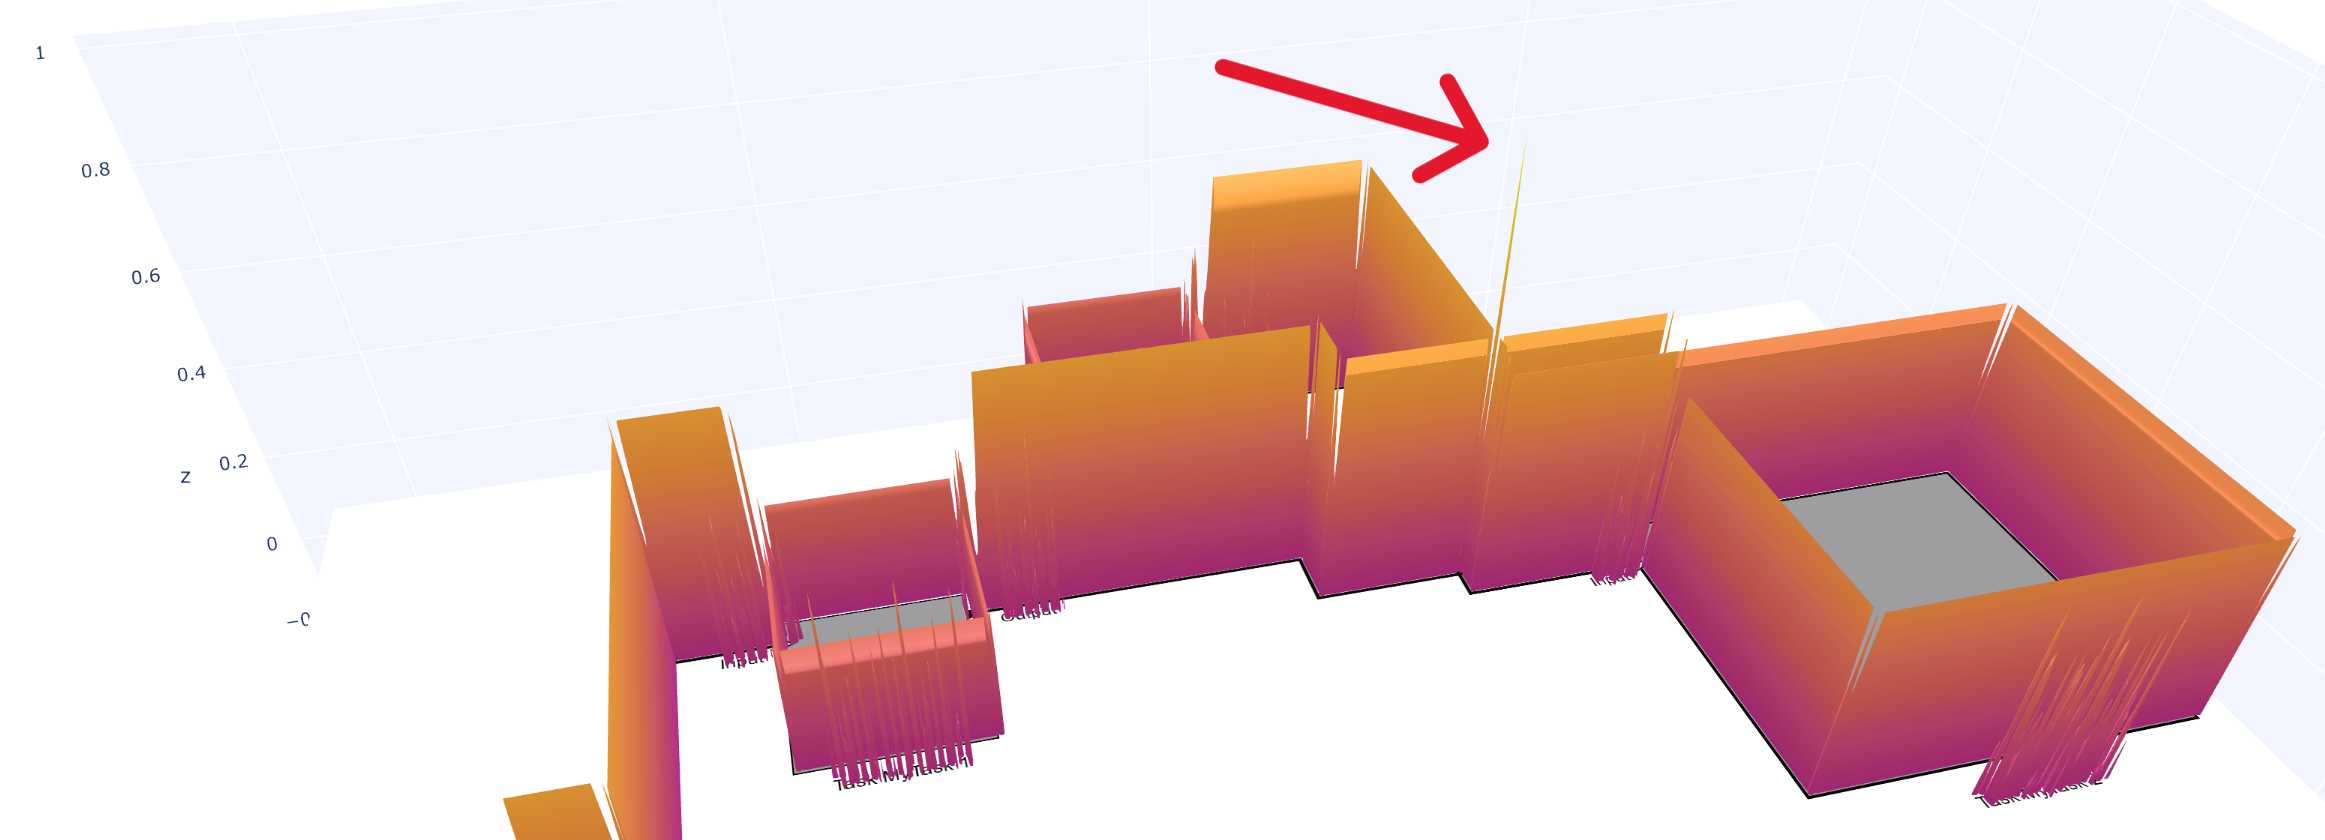
\includegraphics[width=1\linewidth]{Pictures/intersection_peak.png}
    \caption{Peak is visible at intersection}
    \label{fig_intersection_peak}
\end{figure}\\
Misidentified letters and ports are removed by filtering out all line segments with a length shorter than 20 pixels. In all test cases, this approach successfully removes the unwanted line segments while keeping the edges \ref{fig_comparison_filter}.\\
As shown in \ref{fig_threshhold}, the \textit{filter2D()} function initially does not detect any edges at intersections, leading to gaps between the line segments. To process these gaps, it is assumed that intersections always consist of two straight edges. Overlapping 90° turns are considered impossible and will result in an error, forcing the user to maintain a clear diagram structure.\\
First, all intersections in the image are detected using OpenCV's \textit{matchTemplate()} function, which matches a template to overlapping regions of the image (Figure \ref{tm_sqdiff_normed}).\\
The function slides the template across the image, comparing overlapping patches with the template using a specified method. Among the available methods \cite{comparison_methods}, tm\_sqdiff\_normed produced the most accurate results. For each pixel, the function calculates and assigns a value representing the similarity between the template and the corresponding image region. While this approach is more precise than \textit{filter2D()}, it is also significantly more resource-intensive.
\begin{equation}
\label{tm_sqdiff_normed}
    R(x,y) = \frac{\sum_{x', y'}{(T(x', y') - I(x + x', y + y'))^2}}{\sqrt{\sum_{x', y'}{(T(x', y')^2 * \sum_{x', y'}{I(x + x', y + y')^2}}}}
\end{equation}
\begin{wrapfigure}{R}{0.2\textwidth}
\centering
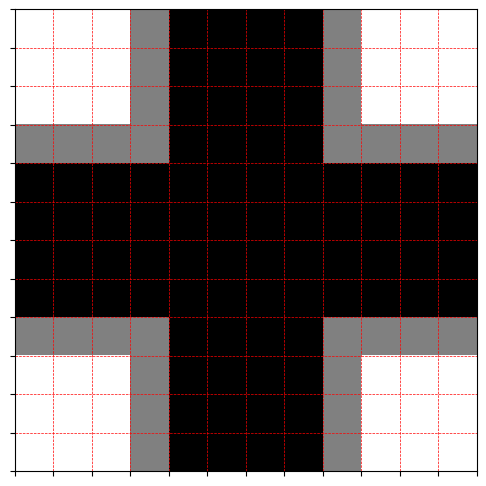
\includegraphics[width=0.2\textwidth]{Pictures/kernel_intersection.png}
\caption{\label{fig_cross}}
% Template used to detect intersections
\end{wrapfigure}
At intersections, the similarity value is approximately 85\%. This slight discrepancy likely arises from how modern operating systems use aliasing to render text and lines with higher apparent resolution and contrast compared to the display. Zooming in reveals that the white pixels near edges are often replaced with subtle color hues or shades of gray \ref{fig_aliasing}. Rendering the results of the template matching highlights a peak in similarity at the intersection (Figure \ref{fig_intersection_peak}). Thresholding isolates this peak, typically yielding two or more matches per intersection. These matches are then filtered based on proximity, ensuring only one match is detected at each intersection.\\
The method processes each detected intersection by connecting the two vertical and two horizontal line segments. This eliminates any residual points near the intersection, leaving only one vertical and one horizontal line segment \ref{fig:_intersection_before_after}.\\
In the allocations editor, the same approach is applied to detect and process signal containers on edges. To enhance diagram readability, it is assumed that no 90° turns are concealed behind the containers and that edges pass through them in a straight line. The primary distinction from intersection detection lies in the number of line segments: at a signal container, only two line segments meet, rather than four.
\begin{figure}[h]
    \centering
    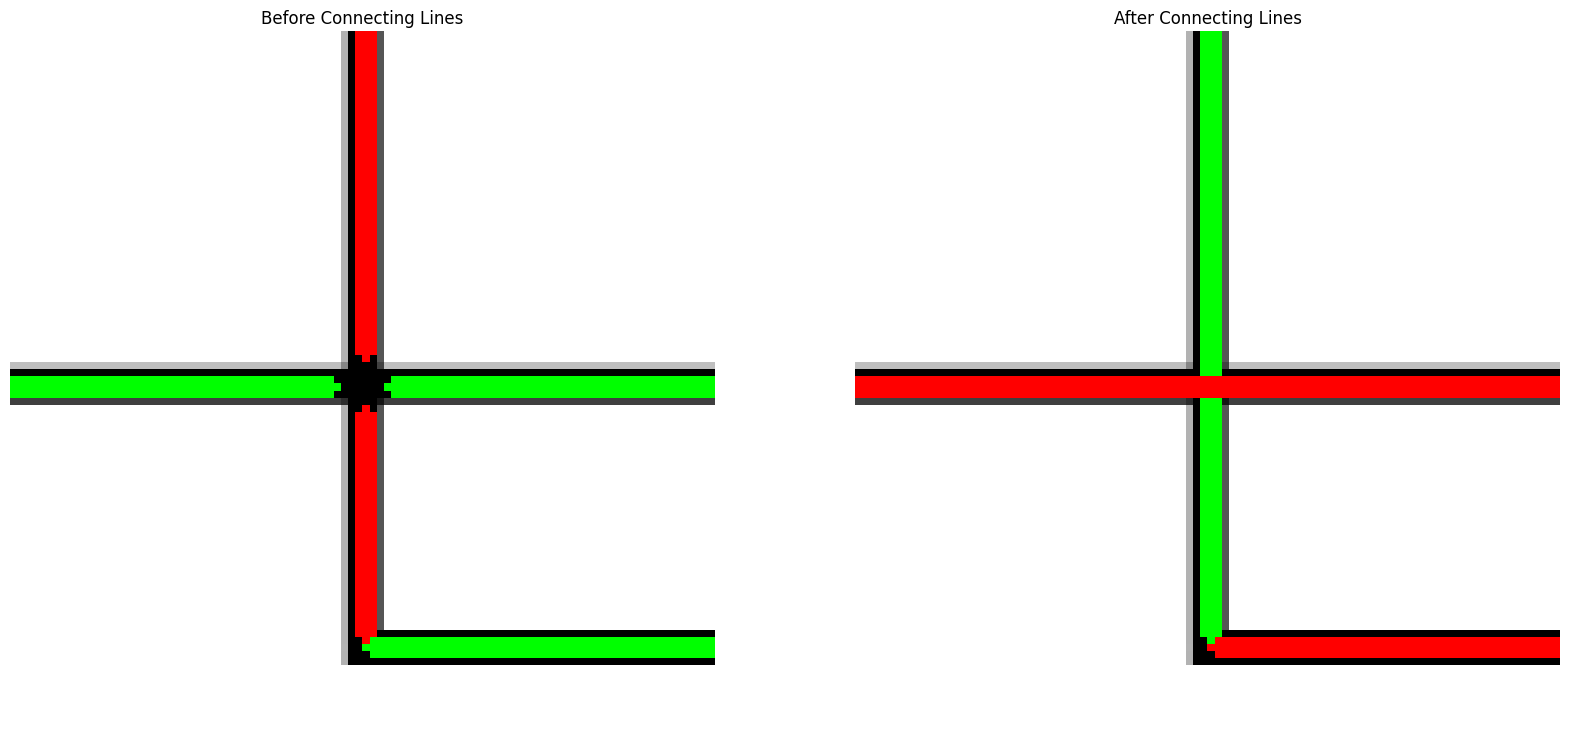
\includegraphics[width=0.7\linewidth]{Pictures/intersection_before_after.png}
    \caption{Intersection before and after connecting the line segments.}
    \label{fig:_intersection_before_after}
\end{figure}\\
Converting the line segments into polylines at this stage would produce unusable data, as the segments are not grouped and not sorted in the sequential order of the edge's \textit{flow}. To generate proper polylines, the line segments must first be sorted into the correct order \ref{fig_line_segment_chains}. For example, if the first line segment in the list is an intermediate line segment within an edge, the polyline function would incorrectly attempt to connect the intermediate points directly to the endpoints, leading to incorrect detections.\\
The implemented method begins by selecting the first line segment, adding it as a starting point to the first chain and to a list of used segments and setting the chain\_growing flag to true. It then iterates through the remaining segments, checking whether each segment has already been used and whether any of its points lie within 7 pixels of the endpoints of the current segment. If a match is found, the segment is added to the used\_segments list and the current chain. If no segment is found within the 7-pixel threshold, the chain\_growing flag is set to false, and the completed chain is added to the list of chains. This process continues until all line segments have been assigned to a chain \ref{fig_chains_before_after}
\begin{figure}[h]
    \centering
    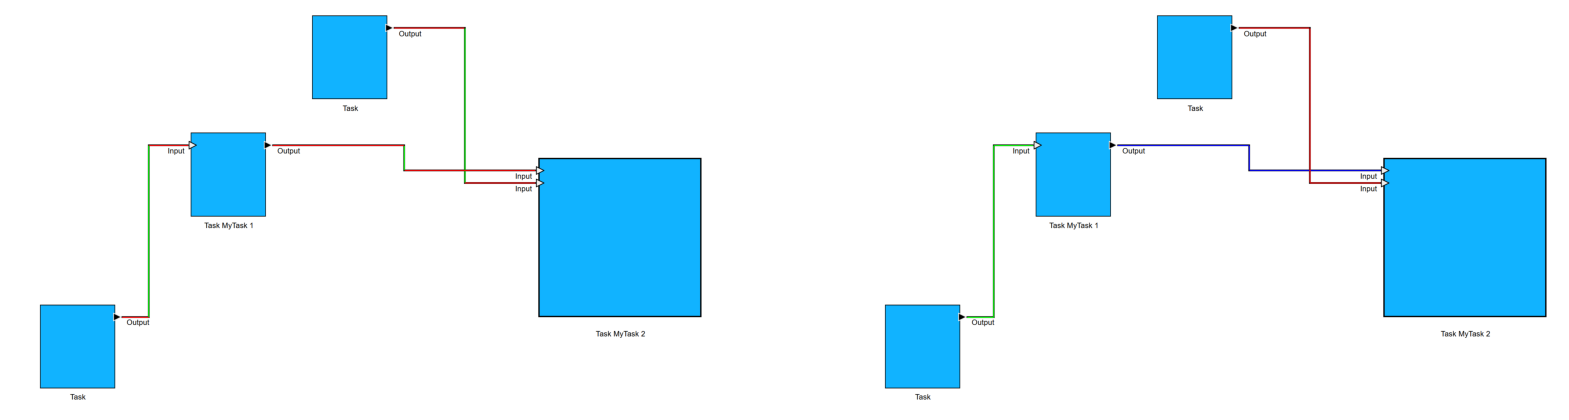
\includegraphics[width=\linewidth]{Pictures/chains_before_after.png}
    \caption{Left: detected vertical and horizontal line segments\\Right: detected line segments processed into colored line segment chains}
    \label{fig_chains_before_after}
\end{figure}\\
Generating the polylines now would yield better results, but still create unusable data, because the line segments within each chain and the two points within each line segment are not sorted. The first point in a list of line segments in a chain could for example be a point in the middle of the chain, resulting in OpenCV's Polyline function to connect the following points in the wrong order.\\
The sorting algorithm for solving this problem has two parts: the first sorts the line segments from beginning of the chain to the end, the second sorts the end- and startpoint of each line segment individually, so that they too appear in order of 'flow' in the chain.

To differentiate between intermediate points and endpoints the function utilizes the way in which the points where found in the first place: when two line segments intersect to form a 90° degree turn, each segment consists of a start- and an endpoint. This means, there are always two points in close proximity at intermediate points, where line segments meet, but only one point at the endpoints, because there is only one line segment ending at each endpoint \ref{fig_zoomed_in_points}.
Using this discrepancy, the function identifies endpoints by iterating through all points and checking for any other points within a five-pixel radius. Any point without any other points within this radius is considered an endpoint of a chain.\\
\begin{figure}
    \centering
    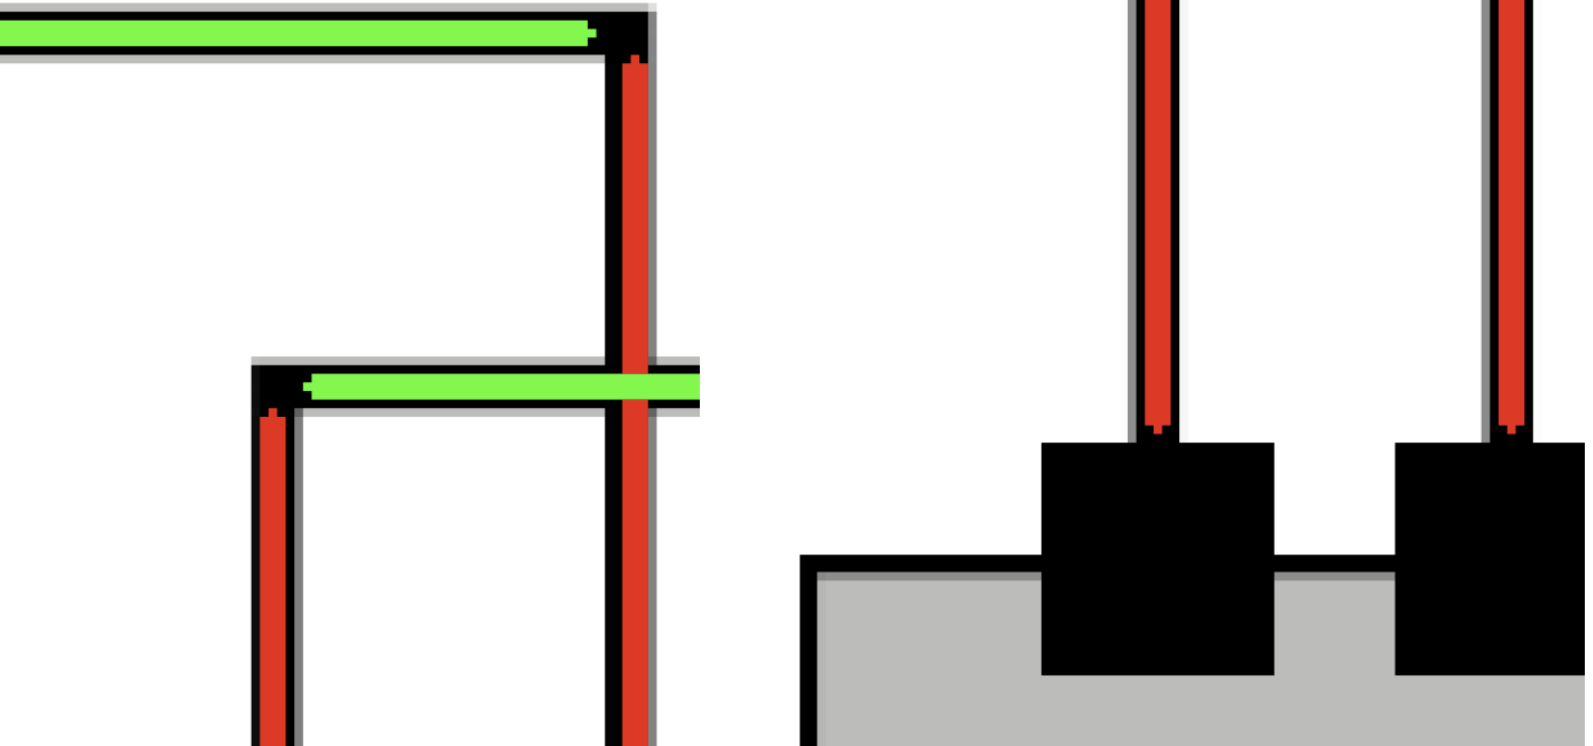
\includegraphics[width=0.5\linewidth]{Pictures/zoomed_in_points.png}
    \caption{Difference between intermediate points and endpoints}
    \label{fig_point_zoom}
\end{figure}
Using the identified endpoints to initialize the sorted\_chain list allows the program to organize the chains systematically. The process begins by selecting the segment that includes one of the start points as the initial segment of the chain. The endpoint of this segment that is not a chain endpoint is designated as the first last\_point in the sorted\_chain list. To determine the next segment in the chain, a lambda function calculates the distance between the last point and both points of each remaining segment. The segment containing the point with the smallest distance to the last\_point is selected as next\_segment and removed from the list of remaining\_segments. Within this segment, the point closest to the last\_point is appended first to the sorted\_chain, followed by the other point of the segment. This process repeats until no segments remain in the remaining\_segments list. The entire process is repeated for each chain until all points in all chains are ordered according to the edge's flow.

To generate polylines, ordered lists of points, from the sorted chains, the method iterates through the sorted\_chains list, appending each point in sequence. Once the polyline is constructed, it is converted into the format required by OpenCV for further processing.
\subsection{Further Improvements}
This method successfully detects and processes nearly all edges within XGEE. In contrast to the previous algorithm, it can identify edges in any orientation, regardless of their start or endpoint or order of their line segments. Furthermore, it is capable of processing and interpreting intersections and signal containers, making it well-suited for handling large, complex models. The method performs reliably across all three editor modes, provided the models are formatted correctly.
A notable problem arises when vertices with surrounding black edges are scaled sufficiently, making their edges resemble signal-carrying edges, which complicates their differentiation. In this case, a possible solution would be to let the vertex detection run first and exclude the found areas when applying the edge detection. Alternatively, the presence of colored pixels around the edges could be checked, as the background around edges is typically white, unlike the areas inside device or function vertices. This way, any obstructions caused by the vertices can be avoided.\\
Another issue may arise if the edges are configured by the user in an unexpected way. For instance, intersection within a few pixels of each other or intersections hidden behind vertices cannot be properly interpreted by the current method, which could lead to unexpected results. Future improvements of the XGEE editor, such as a more advanced automatic arrangement algorithm, could reduce or eliminate the risk of ambiguous user input. Additionally, enhancing the readability of subtask edges within the allocations editor would be beneficial for improving the verification tool. Currently, these edges often overlap with text, are thin and have poor contrast, making them difficult for the current edge detection pipeline to detect accurately.

\section{Vertex Detection}
Vertices represent distinct visual elements within XGEE such as functions, devices, containers or IO ports. Identifying these vertices is critical for interpreting the structural arrangement of diagrams. This section introduces a template-matching approach to address problems including overlapping vertices and varying sizes, ensuring a more reliable vertex detection in all relevant diagram types within XGEE.

A major problem in template matching is the differing occurances of the searched for template in the images. Especially in the allocations editor, there are blue subtasks inside the grey device boxes and blue arrows inside the container. Each of these vertices "contaminates" the underlying vertex and lowers the number of matching pixels in that area. To combat this issue, the subtasks, which are not obscured by other vertices and cannot be resized, are found first using regular template matching. The found bounding boxes are then covered using the same grey color as the surrounding device boxes. This ensures the detection of the devices in the following step works more reliable, independent of the number of subtasks inside the device.\\
for the containers, this approach would work as well, however there is a simpler solution. Because the signal arrows and their attached names tend to be placed in the center of the container, a mask can be used when template matching, to only consider the outer edge of pixels of the container. As long as it has a color different of its surroundings, this approach supplies a simmilar amount of reliablity as the solution used for the subtask detection.

\section{Text Recognition}
The original text detection in XGEE utilized Pytesseract, an open-source optical character recognition (OCR) engine developed and sponsored by Google in 2006. Pytesseract required separate installation from other packages and could only detect text in images that had been preprocessed. Additionally, the output data required extensive postprocessing to become usable. While Pytesseract demonstrated high accuracy and speed, it struggled to reliably detect small text or text with low contrast to the background. Its optimization for structured text formats, such as those found in books, further hindered its performance in XGEE, where text can appear in varying orientations, sizes, and positions. These limitations made reliable text detection using Pytesseract difficult to achieve.
\subsection{Methology}
After evaluating various OCR engines, including EasyOCR [https://pypi.org/project/easyocr/], Doctr [https://pypi.org/project/python-doctr/], and Keras-OCR [https://pypi.org/project/keras-ocr/], EasyOCR proved to be the most suitable alternative.
EasyOCR is a deep-learning-based OCR engine that reliably detects text in images, even under challenging conditions such as low contrast or resolution. Although it operates more slowly on modern CPUs compared to some alternatives, it performs significantly faster on GPUs. Additionally, its ability to detect text in multiple languages adds potential value for future applications. Integration of EasyOCR into the XGEE editor for the user is straightforward, as it can be installed directly via pip install easyocr through the requirements.txt file without requiring additional dependencies or downloads. Unlike Pytesseract, EasyOCR does not necessitate image preprocessing, and it structures found characters into words and sentences automatically based on proximity, eliminating the need for extensive postprocessing. These advantages make EasyOCR the optimal choice for the updated text detection pipeline within XGEE.

First, a reader object is created and the language of the text is specified. The readtext function of the reader object is then called with the image as an argument. The image has to be padded to have a square shape, so there are no problems rotating the data later. This function returns a list of tuples, containing the detected text, its bounding box and a certainty factor. This step is repeated with the rotated image. The positions of the bounding boxes of the found rotated text are then rotated around the center of the image to reallign them with the found text of the original image. Reading an image which contains rotated text usually results in many falsely read characters, because for example 'o' and 'l' can be interpreted regardless of orientation. To filter out the falsely red characters, the algorithm first combines the found results of both ocr-searches and then removes every word shorter than three letters. Because easyocr automatically groups detected characters into words and sentences, this is a simple and effective method to filter out falsely read characters which is able to detect all text in the 10 testcases within this paper. Using this approach also allows the same algorithm to be used for all images, regardless of the XGEE editor they were created in.
\subsection{Future Improvements}
In the future, this method could be improved by using a more advanced algorithm to filter out falsely read characters. and checking the current editor to only search for rotated characters if they are actually present in the image.